% generated by scripts/pkl_to_latex.py
% source PKL : uscan_v1_L6_Ne6_t0p1_mode-uniform_nmin2_solver-gcg_full_es_restarts10_iter300_kmax5_tol1em09_U0.1to5_N21-8081b758e7cc.pkl
% scan type  : uscan
% state      : ex_singlet
% quantity   : linear-entropy
% requires   : \usepackage{pgfplots} \pgfplotsset{compat=1.18}
% colours match the matplotlib PDF (tab10 cycle)
\definecolor{gmeC0}{HTML}{1F77B4}
\definecolor{gmeC1}{HTML}{FF7F0E}
\definecolor{gmeC2}{HTML}{2CA02C}
\definecolor{gmeC3}{HTML}{D62728}
\definecolor{gmeC4}{HTML}{9467BD}
\definecolor{gmeC5}{HTML}{8C564B}
\definecolor{gmeC6}{HTML}{E377C2}
\definecolor{gmeC7}{HTML}{17BECF}

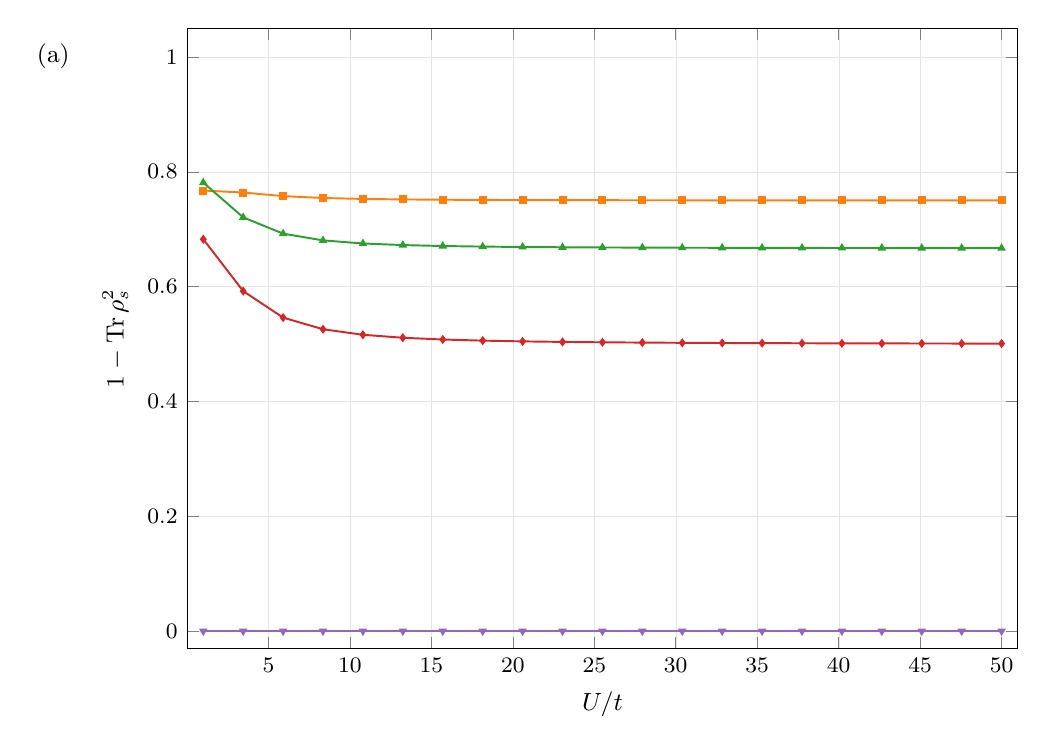
\begin{tikzpicture}
  \begin{axis}[
    width=\columnwidth,
    height=0.78\columnwidth,
    xlabel={$U/t$},
    ylabel={$1-\mathrm{Tr}\,\rho_s^2$},
    grid=both,
    grid style={line width=.1pt, draw=gray!20},
    tick label style={font=\footnotesize\rmfamily, /pgf/number format/fixed},
    label style={font=\small\rmfamily},
    scaled ticks=false,
    legend style={font=\scriptsize\rmfamily, draw=gray!40, at={(0.5,1.03)}, anchor=south, /tikz/every even column/.append style={column sep=6pt}},
    legend cell align={left},
    legend columns=2,
    ymin=-0.03,
    ymax=1.05,
    xmin=0.02,
    xmax=50.98,
    after end axis/.append code={\node[anchor=east, font=\small\rmfamily] at (axis description cs:-0.13,0.954) {(a)};},
  ]
    \addplot[color=gmeC1, mark=square*, mark size=1.1pt, line width=0.7pt] coordinates {
        (1,0.767296) (3.45,0.763883) (5.9,0.757622) (8.35,0.754349)
        (10.8,0.752725) (13.25,0.751847) (15.7,0.751328) (18.15,0.750999)
        (20.6,0.750778) (23.05,0.750623) (25.5,0.75051) (27.95,0.750425)
        (30.4,0.750359) (32.85,0.750308) (35.3,0.750267) (37.75,0.750233)
        (40.2,0.750206) (42.65,0.750183) (45.1,0.750164) (47.55,0.750147)
        (50,0.750133)
    };
    \addplot[color=gmeC2, mark=triangle*, mark size=1.1pt, line width=0.7pt] coordinates {
        (1,0.781223) (3.45,0.7206) (5.9,0.692245) (8.35,0.680517)
        (10.8,0.675144) (13.25,0.672344) (15.7,0.670722) (18.15,0.669704)
        (20.6,0.669026) (23.05,0.668551) (25.5,0.668206) (27.95,0.667948)
        (30.4,0.66775) (32.85,0.667594) (35.3,0.66747) (37.75,0.667369)
        (40.2,0.667286) (42.65,0.667217) (45.1,0.667159) (47.55,0.667109)
        (50,0.667067)
    };
    \addplot[color=gmeC3, mark=diamond*, mark size=1.1pt, line width=0.7pt] coordinates {
        (1,0.682539) (3.45,0.592203) (5.9,0.546046) (8.35,0.52581)
        (10.8,0.516144) (13.25,0.51096) (15.7,0.507899) (18.15,0.505952)
        (20.6,0.504642) (23.05,0.503719) (25.5,0.503046) (27.95,0.50254)
        (30.4,0.502149) (32.85,0.501843) (35.3,0.501597) (37.75,0.501397)
        (40.2,0.501233) (42.65,0.501096) (45.1,0.50098) (47.55,0.500882)
        (50,0.500798)
    };
    \addplot[color=gmeC4, mark=triangle*, mark size=1.1pt, mark options={rotate=180}, line width=0.7pt] coordinates {
        (1,0) (3.45,0) (5.9,0) (8.35,0)
        (10.8,0) (13.25,0) (15.7,0) (18.15,0)
        (20.6,0) (23.05,0) (25.5,0) (27.95,0)
        (30.4,0) (32.85,0) (35.3,-0) (37.75,0)
        (40.2,0) (42.65,0) (45.1,0) (47.55,0)
        (50,0)
    };
  \end{axis}
\end{tikzpicture}
